\subsection*{Data Collection}

A Struck Integrated Systems (SIS) 3302 DAQ module was used to collect data. This module has 16-bit ADCs and an internal 100 MHz clock which was used for all of the measurements. Preamplifier output signals were fed directly to the DAQ module without additional processing. These output signals were digitized and used to perform this analysis. Additionally, the on-board shaping amplifier was used to retrieve event energies (in ADC units).

The trigger threshold value was set so that gamma-ray pulses with energies as low as approximately 50 keV could be collected without excessive noise and without exceeding the voltage range of the DAQ. Data was collected attempting to have negligible pile-up effects. The event rate was chosen to be approximately 800 Hz (triggers) for a system with a 100 MHz clock (10 ns sampling time) and a preamplifier pulse decay time of roughly 50 $\mu$s.

Before further processing each pulse was baseline corrected. This was done by subtracting the average value of the first 15 samples from all of the samples in that pulse.

\subsection*{Energy Calibration}

Before taking spectral data, each channel must be calibrated. The 661.7 keV line from ${}^{137}$Cs and the 59.5 keV line from ${}^{241}$Am were used to perform a linear energy calibration.

Four calibration data sets were taken. First an ${}^{241}$Am source was placed near the outward face of detector 1. Next, the source was moved to the outward source of the detector 2. This was repeated with a ${}^{137}$Cs source. This was done to ensure that all channels would have spectral data for both sources.

Two spectra were plotted for each channel, one using both ${}^{241}$Am data sets combined, and the other using both ${}^{137}$Cs data sets combined. A region of interest around each photopeak was selected by visual inspection of the relevant spectrum. These regions were each fit with a Gaussian function and a linear function (to account for background) using the built in models in LmFit \cite{LMFIT}. A linear energy calibration was used.

Channels which had fewer than 50 total counts around the ${}^{137}$Cs peak or showed other strange behavior (visually observed) in spectra were not calibrated, and were not used in any of the analysis shown. This included 22 of the 152 channels. Most of these channels correspond to strips near the edge of the detectors which have been disconnected due to high leakage currents. The two channels with the highest FWHM values had very few events in the cesium photopeak region, leading to poor fitting. Channels with a 0 FWHM are those which were not calibrated.

The energy resolution of each channel is determined from the FWHM of the peak. This is shown in figure \ref{fwhm}. Each individual channel had a low number of counts in the photopeak ($\approx$ 60). The error bars shown correspond to fitting errors. Low statistics in the cesium peaks limited this procedure (there were roughly 60 counts for a single channel). The average energy resolution was found to be 2.44 keV., with a standard deviation of 0.51 keV. The channels with high FWHM values tend to be those with a small number of counts in the peak. The variation between channels would likely decrease with better statistics.  Using a larger cesium dataset results in a better energy calibration. This was done in \ref{fwhm_long}. The average energy resolution was found to be 2.37 keV., with a standard deviation of 0.39 keV. Ideally, all strips would have the same energy resolution. Realistically, however, we expect that some strips, in particular those on the outer edges of the detector, to have degraded energy resolution. The DC face of detector 1 contains channels 0 through 37. Here we see a u-shaped trend in the energy resolution, potentially demonstrating the effects of higher leakage current near the edges.

\begin{figure}
\begin{centering}
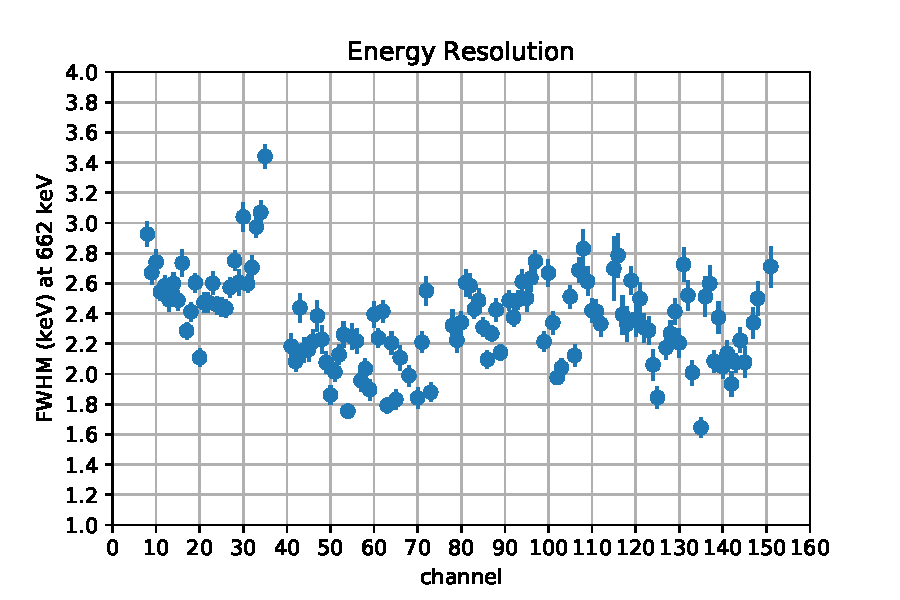
\includegraphics[width=0.7\textwidth]{./figures/energy_res.pdf}
\caption{The energy resolution for each channel of two double-sided strip detectors. Channels with a 0 FWHM are those which were not calibrated due to low statistics, high leakage currents, or other issues. The error bars shown correspond to fitting errors.}
\label{fwhm}
\end{centering}
\end{figure}

\begin{figure}
\begin{centering}
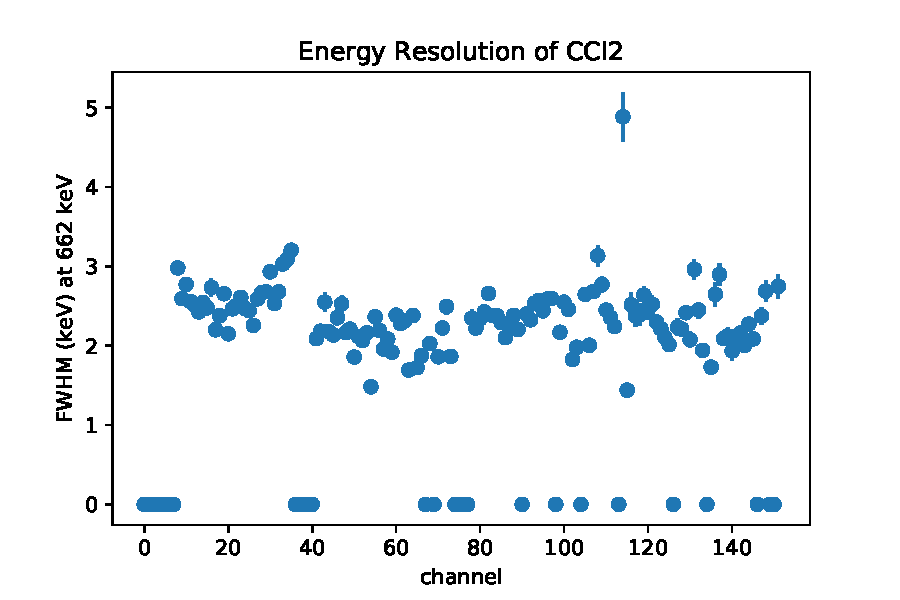
\includegraphics[width=0.7\textwidth]{./figures/energy_res_long.pdf}
\caption{The energy resolution for each channel of two double-sided strip detectors. Channels with a 0 FWHM are those which were not calibrated due to low statistics, high leakage currents, or other issues. The error bars shown correspond to fitting errors.}
\label{fwhm_long}
\end{centering}
\end{figure}

\subsection*{Timing}

A distribution of trigger times over all events and both detectors was plotted. For a Poisson process, the distribution of arrival times is exponential, peaked at zero and falling more steeply with increasing rate (the decay constant of the exponential function is $\lambda = 1/mean rate)$. 

The distribution for experimental triggers does not follow this trend exactly. There are more events near 0 and more events at 1 than at zero. This has to do with the fact that for each event which causes a trigger on a strip, it is very likely to see triggers on other strips (from image charges on neighboring strips, signals from the electrodes on the opposite face or in the other detector, noise, charge-sharing, etc.). It is found that most events occur within 250 nanoseconds of each other. The expected drift time for charges within a detector of this type and size is on the order of hundreds of nanoseconds. This agrees with what is observed. 

\begin{figure}
\begin{centering}
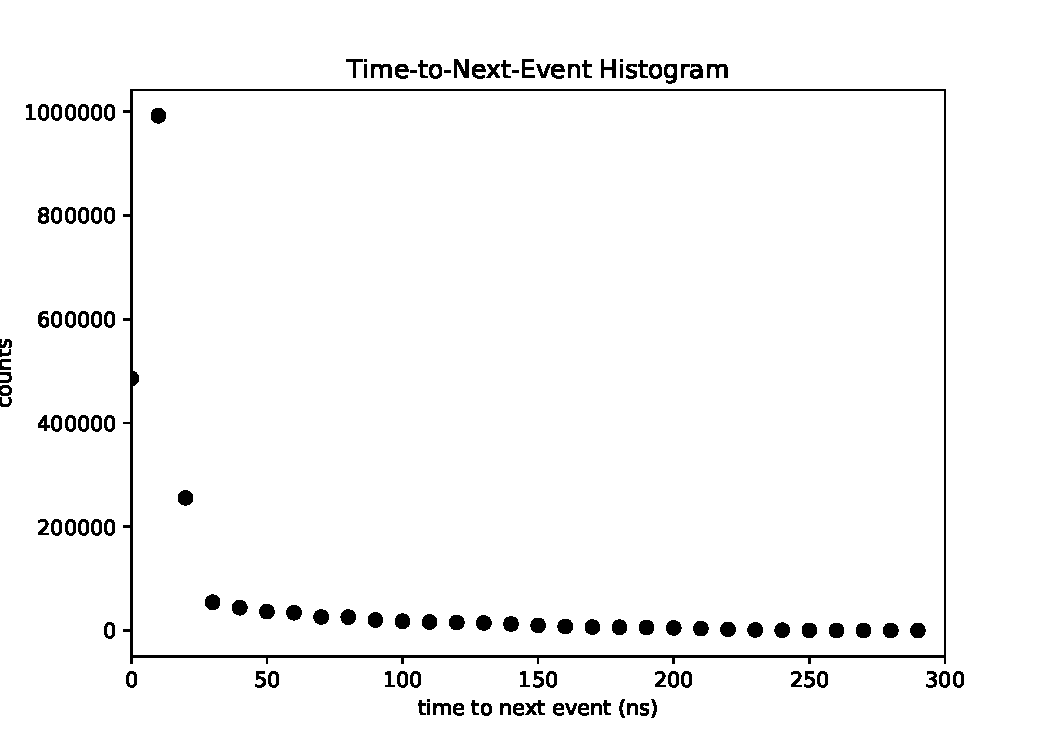
\includegraphics[width=0.7\textwidth]{./figures/time-to-next-event.pdf}
\caption{The energy resolution for each channel. Channels with a 0 FWHM are those which were not calibrated. The error bars shown correspond to fitting errors.}
\label{timehist}
\end{centering}
\end{figure}

To select single-site events, events which have triggers within 400 ns of each other on opposite faces of a detector crystal were selected. This is a generous window, as we expect the drift time for charge carriers within this detector to be $\approx$100-200ns \ref{knoll}. Requiring this, along with full energy deposition, provided the selection criteria for a single-site event.

For an event, each of the two pulses (from the opposite faces) was smoothed using a Savitzky-Golay filter \cite{scipy}. The last point where the smoothed signal did not exceed 50 percent of its maximum value and 6 neighboring points (3 to each side) were fit with a linear function. The time that this linear function crossed 50 percent was calculated and used as $t50$. The $t50$ value of one face was subtracted from the other, to find $\Delta t50$. Here the $t50$ of the electrons was subtracted from that of the holes ($t50_{cathode}- t50_{anode}$). The difference in trigger time was added to $\Delta t50$ to find the difference in signal arrival times.

\begin{figure}
\begin{centering}
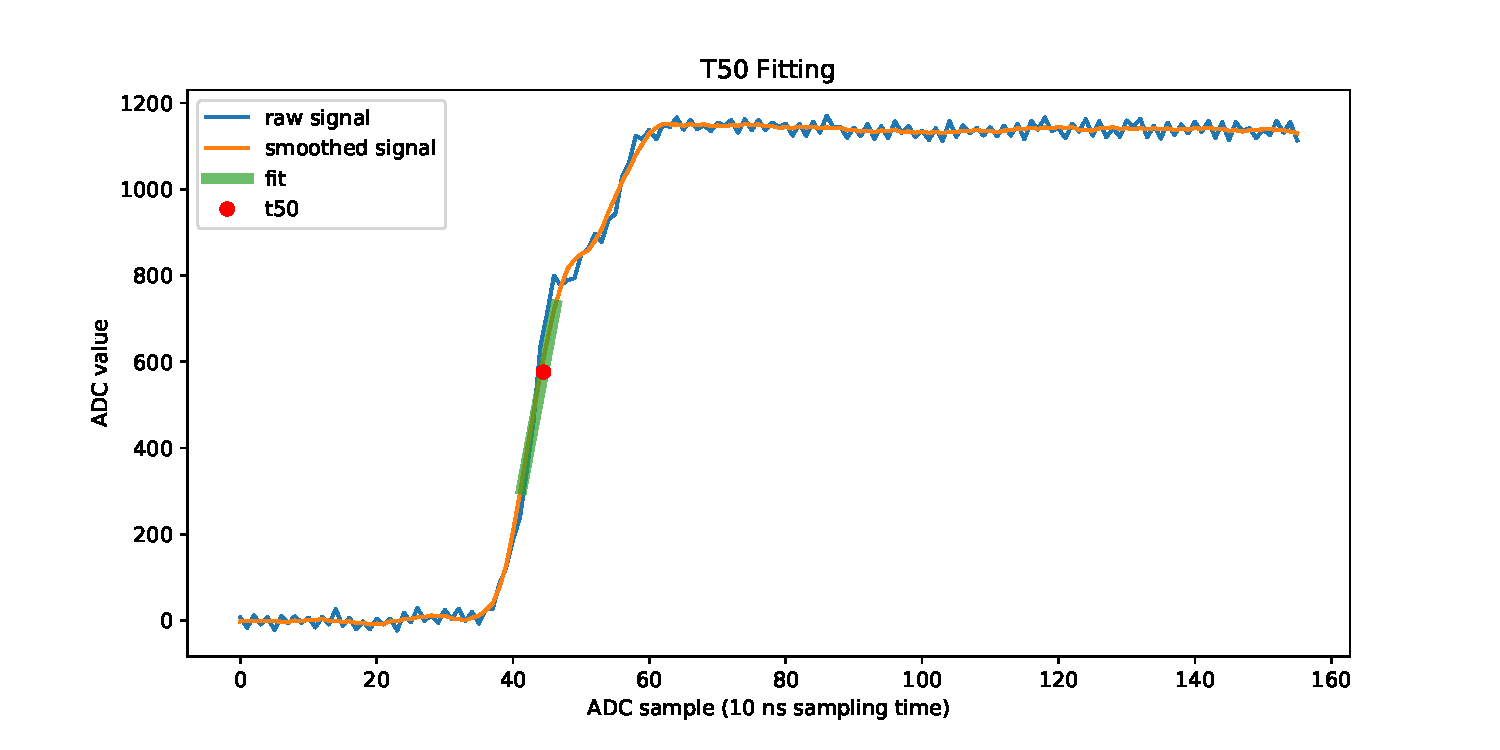
\includegraphics[width=0.7\textwidth]{./figures/t50_fitting.pdf}
\caption{Each raw signal (blue) is smoothed with a Savitzky-Golay filter (orange). The region around the point at which the smoothed signal exceeds half its maximum is fit with a line (green) to extract the t50 value (red point)}
\label{fit}
\end{centering}
\end{figure}

\subsection*{Depth Determination}

${}^{137}$Cs was used to ensure events throughout the potential range of detector depth. Additionally, these signals have greater SNR which makes it easier to properly trigger on and correlate signals.

The maximum $\Delta t50$was seen to be roughly 210, the minimum $\Delta t50$ was seen to be -160. For a rough determination of the depth, the maximum value is assumed to correspond to the anode and the minimum value to the cathode. A linear fit is applied to determine intermediate position values. This is not a fully representative treatment. It fails to take into account effects due to the non-linear weighting potential directly near electrodes, different charge carrier mobilities, realistic charge transport, and other effects. However, for the purposes of this work, we make this crude assumption following \cite{amman}.

A different linear interpretation was used as well. Following \cite{cci21}, assuming saturation velocity for both charge carriers, one can use a linear function to relate depth ($z$) to $\Delta t50$:

\begin{equation}
z = z_0 + k \Delta t50
\end{equation}

where z is the depth of the interaction, $z_0$ is a constant depth which is slightly offset from the midpoint of the detector to account for differences in electron and hole velocities, and $k$ is a proportionality factor. $z_0$ and $k$ were experimentally determined for detector 1 to be 5.2 mm and 0.04 mm/ns respectively, in \cite{cci21}. This offset of 5.2 mm was adjusted to 5.95 mm to better fit the data set.
